In this chapter, we will consider the system of a single particle with mass $\mathcal{M}$, 
position operator $\mathbf{q}$ and momentum operator $\mathbf{p}$.
The particle is placed in a double-well potential, giving the Hamiltionian
%
\begin{equation}\label{DW_hamiltonian}
    \mathbf{H}_{\text{DW}} = \frac{\mathbf{p}^2}{2 \mathcal{M}}  
    + \frac{\mathcal{M}^2 \omega_0^4}{64 \Delta U} \mathbf{q}^4 
    - \frac{\mathcal{M} \omega_0^2}{4} \mathbf{q}^2
    - \mathbf{q} \epsilon .
\end{equation}
%
Here, $\Delta U$ is the barrier height, $\omega_0$ is the classical oscillation frequency
and $\epsilon$ is the bias factor of the double-well potential.
In addition, we introduce a single cavity mode, which couples linearly to the doublet-doublet
system and is described by
%
\begin{equation}
    \mathbf{H}_{C,\text{int}} = \Omega \mathbf{a}^{\dagger} \mathbf{a}
    + g \mathbf{q} \left( \mathbf{a} + \mathbf{a}^{\dagger} \right) .
\end{equation}
%
Next, the cavity mode is coupled to a bath consisting of simple harmonic oscillators. 
For now, we will neglect the direct coupling of the DW-system to a bath:
%
\begin{equation}
    \mathbf{H}_{B,\text{int}} = \left( \mathbf{a} + \mathbf{a}^{\dagger} \right)
    \sum_{k}^{} \nu_k \left( \mathbf{b}_k + \mathbf{b}^{\dagger}_k  \right) 
    + \sum_{k}^{} \omega_k \mathbf{b}^{\dagger}_k  \mathbf{b}_k  .
\end{equation}
%
For the cavity mode, we choose Ohmic damping. In the continuous limit, this means the 
spectral density is given by
%
\begin{equation}
    J_{\text{Ohm}} \left( \omega \right) = \sum_{k}^{} \nu_k^2 \delta\left( \omega - \omega_k \right) 
    = \kappa \omega e^{- \omega / \omega_c} ,
\end{equation}
%
where $\kappa$ is the cavity damping constant and $\omega_c$ is the cut-off frequency. \\
According to Garg, Onuchic and Ambegaokar, this model can be mapped to a double-well 
coupling to a bath with a peaked spectral density with the coupling term
%
\begin{equation}
    \mathbf{H}_{B,\text{DW}} = \mathbf{q} \sum_{k}^{} \lambda_k \left( \tilde{\mathbf{a}}_k  + \tilde{\mathbf{a}}^\dagger_k  \right) 
    + \sum_{k}^{}\tilde{\omega}_k \tilde{\mathbf{a}}^\dagger_k  \tilde{\mathbf{a}}_k  .
\end{equation}
%
and the effective bath spectral density
%
\begin{equation}\label{bath_spectral_density}
    J \left( \omega \right) = \sum_{k}^{} \lambda_k^2 \delta\left( \omega - \tilde{\omega}_k \right) 
    = \frac{2 \alpha \omega \Omega^4}{ \left( \Omega^2 - \omega^2 \right)^2  + \left( 2 \pi \kappa \omega \Omega  \right)^2 } ,
\end{equation}
%
where $\alpha = 8 \kappa g^2 / \Omega^2$ is the effective low-frequency damping constant.
In the low-frequence limit, i.e. $\omega \rightarrow 0$, the effective bath spectral
density reduces to $J \left( \omega \right) \rightarrow 2 \alpha \omega$.

\section{The DW-system in the DVR-basis}

Now, we will calculate the form of the single double-well Hamiltionian (\ref{DW_hamiltonian})
in the DVR-basis. For clarity, we first introduce dimensionless quantities according to 
%
\begin{align}
    \tilde{\mathbf{q}} &= \sqrt{\frac{\mathcal{M}\omega_0}{\hbar}}\mathbf{q}, \ \ \ \ \ \tilde{t} = \omega_0 t, \ \ \ \ \ \tilde{T} = \frac{k_B}{\hbar \omega_0} T \\
    \tilde{\Omega} &= \frac{\Omega}{\omega_0}, \ \ \ \ \ E_b = \frac{\Delta U}{\hbar\omega_0}, \ \ \ \ \ \tilde{\epsilon} = \sqrt{\frac{1}{\mathcal{M}\hbar\omega_0}}\epsilon .
\end{align}
%
The Hamiltonian, in units of $\hbar\omega_0$, now reads
%
\begin{equation}
    \tilde{\mathbf{H}}_{\text{DW}} = \frac{\tilde{\mathbf{p}}^2}{2} \\
    + \frac{1}{64 E_b}\tilde{\mathbf{q}}^4 - \frac{1}{4}\tilde{\mathbf{q}}^2 \\
    - \tilde{\epsilon}\tilde{\mathbf{q}}.
\end{equation}
%
From now on, we will drop the tildes and only use the rescaled, dimensionless
quantities. To obtain the eigenvalues of the position operator and the matrix elements
of the double-well Hamiltonian, the procedure described next is peformed. Using the 
eigenstates $\{ \ket{i} \}$ of the simple harmonic oscillator and expressing the position 
and momentum operators in terms of ladder operators, it is possible to calculate the matrix
elements $H_{\text{DW},mn}^{\text{SHO}}=\bra{m}\mathbf{H}_{\text{DW}}\ket{n}$,
which is in principle an infinite-dimensional square matrix. Since we are mostly interested in the 
lowest four energy levels, we choose to only keep the $K\times K$ submatrix consisting
of the first $K$ rows and column. Naturally, we have to choose $K$ large enough such
that the smallest four eigenvalues have converged sufficiently close to their asymptotic value.
The resulting $K\times K$ matrix can then be diagonalized using standard analytical or
numerical methods, returning $K$ energy eigenvalues $\{\mathcal{E}_1,\mathcal{E}_2,...,\mathcal{E}_K\}$
and eigenvectors $\{\Psi_1,\Psi_2,...,\Psi_K\}$. The diagonalized matrix is then obtained as 
%
\begin{equation}
    \mathbf{H}_{\text{DW}}^{\text{Eig}} = M_{\text{SHO}\rightarrow\text{Eig}} 
    \mathbf{H}_{\text{DW}}^{\text{SHO}} M_{\text{SHO}\rightarrow\text{Eig}}^{-1}
    = \text{diag}(\mathcal{E}_1,\mathcal{E}_2,...,\mathcal{E}_K),
\end{equation}
%
with $M_{\text{SHO}\rightarrow\text{Eig}}$ being basis transformation matrix whose $k$-th 
column is the $k$-th eigenvector $\ket{\Psi_k}$ in the SHO-basis.
Having determined the first $K$ eigenenergies to sufficient precision, we now only keep
the four lowest energy eigenstates such that
%
\begin{equation}
    \mathbf{H}_{\text{DW}}^{\text{Eig}} = \text{diag}(\mathcal{E}_1,\mathcal{E}_2,\mathcal{E}_3,\mathcal{E}_4).
\end{equation}
%
Because we are interested in the evolutions of populations of the left and right side
of the wells, we switch to the localized basis defined by
%
\begin{align}
    \ket{L_1} &= \frac{1}{\sqrt{2}} \left( \ket{\psi_1} - \ket{\psi_2} \right), \ \ \ \ \ \ket{R_1} = \frac{1}{\sqrt{2}} \left( \ket{\psi_1} + \ket{\psi_2} \right), \\
    \ket{L_2} &= \frac{1}{\sqrt{2}} \left( \ket{\psi_3} - \ket{\psi_4} \right), \ \ \ \ \ \ket{R_2} = \frac{1}{\sqrt{2}} \left( \ket{\psi_3} + \ket{\psi_4} \right).
\end{align}
%
From this definition the basis transformation matrix can be read off to be
%
\begin{equation}
    M_{\text{Eig}\rightarrow\text{Loc}} = \frac{1}{\sqrt{2}}
    \begin{pmatrix}
        1 & -1 & 0 & 0 \\
        1 & 1 & 0 & 0 \\
        0 & 0 & 1 & -1 \\
        0 & 0 & 1 & 1 
    \end{pmatrix},
\end{equation}
%
and as before, the Hamiltonian in the localized basis is 
%
\begin{align}
    \mathbf{H}_{\text{DW}}^{\text{Loc}} &= M_{\text{Eig}\rightarrow\text{Loc}} 
    \mathbf{H}_{\text{DW}}^{\text{Eig}} M_{\text{Eig}\rightarrow\text{Loc}}^{-1} \\
    &= \sum_{i=1,2} \left[ \bar{\mathcal{E}}_i 
    (\ket{L_i}\bra{L_i}+\ket{R_i}\bra{R_i}) - \frac{\Delta_i}{2}(\ket{L_i}\bra{R_i}+\ket{R_i}\bra{L_i})\right],
\end{align}
%
with $\bar{\mathcal{E}}_1 = (\mathcal{E}_1+\mathcal{E}_2)/2$, $\bar{\mathcal{E}}_2 = (\mathcal{E}_3+\mathcal{E}_4)/2$, 
$\Delta_1 = \mathcal{E}_2- \mathcal{E}_1$ and $\Delta_2 = \mathcal{E}_4- \mathcal{E}_3$.
One can verify that $\bra{\psi_i}\mathbf{q}\ket{\psi_j}=\bra{\psi_j}\mathbf{q}\ket{\psi_i}$
and that further $\bra{\psi_1}\mathbf{q}\ket{\psi_3}=\bra{\psi_2}\mathbf{q}\ket{\psi_4}=0$,
such that one can write the position operator $\mathbf{q}$ in the localized basis as
%
\begin{align}
    \mathbf{q}^{\text{Loc}} &= q_{12} ( \ket{R_1}\bra{R_1} -
    \ket{L_1}\bra{L_1}) + q_{34} ( \ket{R_2}\bra{R_2} -
    \ket{L_2}\bra{L_2} ) \\
    &+ \frac{q_{12}+q_{34}}{2}( \ket{R_1}\bra{R_2}+\ket{R_2}\bra{R_1}-\ket{L_1}\bra{L_2}-\ket{L_2}\bra{L_1} ) \\
    &+ \frac{q_{12}-q_{34}}{2}( \ket{R_2}\bra{L_1}+\ket{L_1}\bra{R_2}-\ket{L_2}\bra{R_1}-\ket{R_1}\bra{L_2} )
\end{align}
%



Using the representation of the momentum and position operators in terms
of the ladder operators of the simple harmonic oscillator,
%
\begin{equation}
    \mathbf{q} = \frac{1}{\sqrt{2}} ( \mathbf{a} + \mathbf{a}^\dagger ), \ \ \ \ \ \\
    \mathbf{p} = \frac{1}{\sqrt{2}\text{i}} ( \mathbf{a} - \mathbf{a}^\dagger ),
\end{equation}
%
we can compute the matrix elements of the Hamiltonian in the SHO basis to be
\begin{align}
    \langle m | \mathbf{H}^{\text{SHO}}_{\text{DW}} | n \rangle
    &= \frac{1}{8} \left[ (2n+1)\delta_{m,n} -3\sqrt{n(n-1)}\delta_{m,n-2}
    - 3\sqrt{(n+1)(n+2)}\delta_{m,n+2} \right] \\
    &+ \frac{1}{256E_b} \left[ \sqrt{n(n-1)(n-2)(n-3)}\delta_{m,n-4}+2(2n-1)\sqrt{n(n-1)}\delta_{m,n-2} \right.\\ 
    &+ \left. 3(2n^2+2n+1)\delta_{m,n} + 2(2n+3)\sqrt{(n+1)(n+2)}\delta_{m,n+2} \right. \\
    &+ \sqrt{(n+1)(n+2)(n+3)(n+4)}\delta_{m,n+4} \left. \vphantom{\sqrt{(1)}}\right].
\end{align}
%
We then take the submatrix conisting of the first $K\in\mathbb{N}$ rows and columns of 
$\mathbf{H}^{\text{SHO}}_{\text{DW}}$ and diagonalize it. Since $K$ has to be chosen such 
that the resulting eigenvalues have converged closely to their actual values and is thus 
relatively large (e.g. $K=50$), this has to be done numerically. This yields a set of 
eigenenergies $\{\mathcal{E}_1,\mathcal{E}_2,...,\mathcal{E}_K\}$ and corresponding 
eigenvectors 
%
\begin{equation}
    \ket{\psi_i} = \sum_{k=0}^{K-1} c_k^{(i)} \ket{k},
\end{equation}
%
with $\ket{k}$ being the $k$-th SHO eigenstate and $c_k^{(i)}$ being the entry in the 
$i$-th row and $k$-th column of the basis transformation matrix. Now, we restrict our system
to its four lowest energy eigenstates and perform a further basis transformation to
the so-called localized basis defined by
%
\begin{align}
    \ket{L_1} &= \frac{1}{\sqrt{2}} \left( \ket{\psi_1} - \ket{\psi_2} \right), \ \ \ \ \ \ket{R_1} = \frac{1}{\sqrt{2}} \left( \ket{\psi_1} + \ket{\psi_2} \right), \\
    \ket{L_2} &= \frac{1}{\sqrt{2}} \left( \ket{\psi_3} - \ket{\psi_4} \right), \ \ \ \ \ \ket{R_2} = \frac{1}{\sqrt{2}} \left( \ket{\psi_3} + \ket{\psi_4} \right).
\end{align}
% 
The Hamiltonian in the localized basis can be determined by basic matrix algebra, eventually 
giving
%
\begin{equation}
    \mathbf{H}^{\text{LOC}}_{\text{DW}} = \sum_{i=1,2} \left[ \bar{\mathcal{E}}_i \\
    (\ket{L_i}\bra{L_i}+\ket{R_i}\bra{R_i}) - \frac{\Delta_i}{2}(\ket{L_i}\bra{R_i}+\ket{R_i}\bra{L_i})\right],
\end{equation}
%
where $\bar{\mathcal{E}}_1 = (\mathcal{E}_1+\mathcal{E}_2)/2$, $\bar{\mathcal{E}}_2 = (\mathcal{E}_3+\mathcal{E}_4)/2$,
$\Delta_1 = \mathcal{E}_2-\mathcal{E}_1$ and $\Delta_2 = \mathcal{E}_4-\mathcal{E}_3$.

\section{Calculation of the Rate Matrix Elements}

The Markov-approximated rate matrix elements read, to lowest order, 
%
\begin{equation}\label{rate_matrix_elements}
    \Gamma_{\mu\nu}^{(2)} = \frac{\Delta_{\mu\nu}^2}{2} \int_{0}^{\infty} \text{d} \tau 
    e^{- \left( q_\mu - q_\nu \right)^2 S \left( \tau \right)} \cos \left[ \left( E_\mu - E_\nu \right) 
    \tau + \left( q_\mu - q_\nu \right)^2 R \left( \tau \right) \right] ,
\end{equation}
%
where $S(\tau)$ and $R(\tau)$ are the real and complex parts of the twice integrated bath
autocorrelation function reading
%
\begin{equation}
    Q \left( \tau \right) = S \left( \tau \right) + \text{i} R \left( \tau \right) 
    = \frac{1}{\pi} \int_{0}^{\infty} \text{d}\omega \frac{J \left( \omega \right)}{\omega^2}
    \coth\frac{\hbar\omega\beta}{2} \Bigl[ \left( 1-\cos\omega\tau \right) + \text{i}\sin\omega\tau \Bigr].
\end{equation}
%
Again, as in the section before, we use dimensionless quantities as defined previously, 
in addition of $\tilde{\Gamma}=\Gamma/\omega_0$. 
Inserting the bath spectral density (\ref{bath_spectral_density}) and defining
the width of the peaked bath spectral density, $\Gamma = 2 \pi \kappa \Omega$, one obtains the integral
%
\begin{equation}
    S \left( \tau \right) + \text{i} R \left( \tau \right) = \frac{2 \alpha}{\pi} 
    \int_{0}^{\infty} \text{d}\omega \frac{1}{\omega} \frac{\Omega^4}{\left(\Omega^2-\omega^2\right)^2
    + \left(\Gamma\omega\right)^2}
    \coth\frac{\hbar\omega\beta}{2} \Bigl[ \left( 1-\cos\omega\tau \right) + \text{i}\sin\omega\tau \Bigr] .
\end{equation}
%
We will now evaluate the real and complex part of the integral seperately. The real part reads
%
\begin{equation}
    S \left( \tau \right) = \frac{2 \alpha}{\pi} 
    \int_{0}^{\infty} \text{d}\omega \frac{1}{\omega} \frac{\Omega^4}{\left(\Omega^2-\omega^2\right)^2
    + \left(\Gamma\omega\right)^2}
    \coth\frac{\hbar\omega\beta}{2} \left( 1-\cos\omega\tau \right).
\end{equation}
%
Using the symmetry of the integrand with respect to $\omega \rightarrow -\omega$, one can 
rewrite the integral as 
%
\begin{equation}
    S \left( \tau \right) = \frac{\alpha}{\pi} 
    \int_{-\infty}^{\infty} \text{d}\omega \frac{1}{\omega} \frac{\Omega^4}{\left(\Omega^2-\omega^2\right)^2
    + \left(\Gamma\omega\right)^2}
    \coth\frac{\hbar\omega\beta}{2} \left( 1-e^{\text{i}\omega\tau} \right).
\end{equation}
%
This expression is best solved using the residue theorem. For this, we need to determine
the poles of the integrand. The first factor only as a pole of order 1 at $\omega_0 = 0$.
To find the poles of the second factor, one has to solve the equation
%
\begin{equation}
    \left(\Omega^2-\omega^2\right)^2
    + \left(\Gamma\omega\right)^2 = 0 .
\end{equation}
%
Solving this equation is easily performed by simple algebra and yields the following simple poles:
%
\begin{equation}
    \omega_{1,2,3,4} = \pm \frac{\text{i} \Gamma}{2} \pm \sqrt{\frac{\Gamma^2}{4} + \Omega^2}
    = \pm \bar{\Omega} \pm \frac{\text{i} \Gamma}{2},
\end{equation}
%
after defining $\bar{\Omega} = \sqrt{\Gamma^2/4 + \Omega^2}$.
Turning to the third factor, we recall the fact that the hyperbolic cotangent has simple poles
at $x = \text{i} k \pi$, $k \in \mathbb{Z}$. After some calculation, the poles of $\coth\left(\hbar\omega\beta / 2\right)$
are resolved to be
%
\begin{equation}
    \omega = \text{i} \frac{2\pi k}{\hbar\beta} = \text{i} \nu_k, \ k \in \mathbb{Z},
\end{equation}
%
where the $\nu_k$ are the so-called bosonic Matsubara frequencies. As the fourth factor 
does not possess any poles, we have now identified every pole exhibited by the integrand.
Next, we have to choose a suitable integration contour. Here, we choose the half annulus lieing
in the upper complex half-plane with outer radius $R$ and inner radius $r$.
Using this contour, the real part of the bath autocorrelation function is given by
%
\begin{equation}
    \int_{-\infty}^{\infty} \text{d}\omega F(\omega) = 2\pi\text{i}\sum_{k} \text{Res}(F,\omega_k)
    -\lim_{R\rightarrow\infty} \int_{\mathcal{C}_1}\text{d}\omega F(\omega)
    -\lim_{r\rightarrow 0} \int_{\mathcal{C}_2}\text{d}\omega F(\omega),
\end{equation}
%
where $\mathcal{C}_1$ is the outer half-circle and $\mathcal{C}_2$ is the inner half-circle
of the contour and the $\omega_k$ denote the poles of the integrand. In the limit $R\rightarrow\infty$
and $r\rightarrow 0$, we will pick-up all of the poles which lie in the upper complex half-plane,
namely $\omega_1, \ \omega_2$ and $\text{i}\nu_n$ for $n > 0$. Performing the calculation 
of the residues and limits with some care results in
%
\begin{equation}
    S \left( \tau \right) = X\tau + L \Bigl( e^{-(\Gamma/2)\tau} \cos\bar{\Omega}\tau -1 \Bigr)
    + Z e^{-(\Gamma/2)\tau} \sin\bar{\Omega}\tau + S_{\text{Mats}}(\tau),
\end{equation}
%
with the prefactors being
%
\begin{equation}
    L = \frac{\alpha}{\Gamma\bar{\Omega}} \frac{1}{\cosh(\hbar\beta\bar{\Omega})-\cos(\hbar\beta\Gamma/2)}
    \left[ \left( \frac{\Gamma^2}{4}-\bar{\Omega}^2 \right) \sinh(\hbar\beta\bar{\Omega})
    + \Gamma\bar{\Omega} \sin(\hbar\beta\Gamma/2)  \right],
\end{equation}
%
\begin{equation}
    Z = \frac{\alpha}{\Gamma\bar{\Omega}} \frac{1}{\cosh(\hbar\beta\bar{\Omega})-\cos(\hbar\beta\Gamma/2)}
    \left[ -\Gamma\bar{\Omega} \sinh(\hbar\beta\bar{\Omega})
    + \left( \frac{\Gamma^2}{4}-\bar{\Omega}^2 \right) \sin(\hbar\beta\Gamma/2)  \right],
\end{equation}
%
and $X=2\alpha/(\hbar\beta)$. The last term $S_{\text{Mats}}(\tau)$ reads
%
\begin{equation}
    S_{\text{Mats}}(\tau) = -\frac{4\alpha\Omega^4}{\hbar\beta}
    \sum_{n=1}^{\infty}\frac{1}{(\Omega^2+\nu_n^2)^2-\Gamma^2\nu_n^2}
    \left[ \frac{e^{-\nu_n\tau}-1}{\nu_n} \right].
\end{equation}
%
Choosing the same contour for the integration of the imaginary part of (\ref{bath_spectral_density}),
%
\begin{align}
    R(\tau) &= \frac{2 \alpha}{\pi} 
    \int_{0}^{\infty} \text{d}\omega \frac{1}{\omega} \frac{\Omega^4}{\left(\Omega^2-\omega^2\right)^2
    + \left(\Gamma\omega\right)^2}\sin\omega\tau \\
    &= \frac{\alpha}{\pi} 
    \int_{-\infty}^{\infty} \text{d}\omega \frac{1}{\omega} \frac{\Omega^4}{\left(\Omega^2-\omega^2\right)^2
    + \left(\Gamma\omega\right)^2}e^{\text{i}\omega\tau},
\end{align}
%
the imaginary part can be analogously computed to be
%
\begin{equation}
    R(\tau) = \alpha - \alpha e^{-(\Gamma/2)\tau} \left( N\sin\bar{\Omega}\tau +\cos\bar{\Omega}\tau \right),
\end{equation}
%
where $N=(\Gamma^2/4-\bar{\Omega}^2)/(\Gamma\bar{\Omega})$. In order to obtain an analytical
expression for the rate matrix elements, we will now make the assumption that the bath 
spectral density is sharply peaked, which means that $\kappa=\Gamma/(2\pi\Omega)\ll1$.
This allows us to expand the bath correlation function $Q(\tau)$ to the first-order in $\kappa$.
After performing the expansion, we obtain
%
\begin{align}
    S(\tau) &= Y(\cos \Omega \tau - 1)+A \tau \cos \Omega \tau +B \tau \sin \Omega \tau
    + \mathcal{O}\left[\kappa^2\right], \\
    R(\tau) &= W\sin\Omega\tau+V(1-\cos\Omega\tau-\frac{\Omega}{2}\tau\sin\Omega\tau)
    + \mathcal{O}\left[\kappa^2\right],
\end{align}
%
with the temperature dependent coefficients
%
\begin{align}
    Y &= -\frac{4g^2}{\Omega^2}\coth\frac{\hbar\beta\Omega}{2}, \ \ \ W = \frac{4g^2}{\Omega^2} \\
    A &= \frac{4\Gamma g^2}{2\Omega^2}\coth\frac{\hbar\beta\Omega}{2}, \ \ \ B = \frac{8\Gamma g^2}{\Omega^2\hbar\beta} \\
    C &= -\frac{2\Gamma g^2}{\Omega^3}\frac{\hbar\beta\Omega +2\sinh\hbar\beta\Omega}{\cosh\hbar\beta\Omega-1}, \ \ \ V = \frac{4\Gamma g^2}{\Omega^3}.
\end{align}
%
We now turn to the computation of the rate matrix elements.
Inserting the real and imaginary parts of the bath correlation function into (\ref{rate_matrix_elements}),
we obtain
%
\begin{equation}
\begin{split}
    \Gamma_{\mu\nu}^{(2)} = \frac{\Delta_{\mu\nu}^2}{2} \int_{0}^{\infty} \text{d} & \tau 
    \exp \Bigl\{-q_{\mu\nu}^2 Y(\cos\Omega\tau-1) -q_{\mu\nu}^2 A\tau\cos\Omega\tau
    - q_{\mu\nu}^2 B\tau\cos\Omega\tau \Bigr\} \\
    & \times \cos \Bigl\{ E_{\mu\nu} \tau + q_{\mu\nu}^2 W\sin\Omega\tau + 
    V \Bigl( 1-\cos\Omega\tau -\frac{\Omega}{2}\tau \sin\Omega\tau \Bigr) \Bigr\},
\end{split}
\end{equation}
%
where we have introduced for clarity $q_{\mu\nu}=q_\mu - q_\nu$ and $E_{\mu\nu}=E_\mu - E_\nu$.
After using Euler's formula for the cosine and some rearrangement, we arrive at
%
\begin{equation}
    \Gamma_{\mu\nu}^{(2)} = \frac{\Delta_{\mu\nu}^2}{4} e^{ \bar{Y} + \text{i} \bar{V}} \int_{0}^{\infty} \text{d}\tau
    e^{- \bar{B} \tau -\bar{A} \tau \cos\omega\tau}
    e^{\text{i}E_{\mu\nu}\tau-\text{i}\bar{V} \frac{\Omega}{2} \tau\sin\omega\tau}
    e^{(-\bar{Y}-\text{i}\bar{V})\cos\omega\tau}
    e^{(-\bar{C}+\text{i}\bar{W})\sin\omega\tau} + \text{c.c}
\end{equation}
%
after having absorbed the $q_{\mu\nu}^2$ into the barred time-independent factors and denoting
the complex conjugate of the first summand as c.c. Notice that the integral converges
if the condition $\bar{B}>\bar{A}$ is fulfilled, which imposes
%
\begin{equation}
    \frac{4}{\hbar\beta\Omega}>\coth\frac{\hbar\beta\Omega}{2}.
\end{equation}
%
When this requirement holds, we can make further approximations. First, we linearize
%
\begin{align}
    e^{ -\bar{A} \tau \cos\omega\tau} &\approx 1-\bar{A}\tau\cos\omega\tau \\
    e^{-\text{i}\bar{V} \frac{\Omega}{2} \tau\sin\omega\tau} &\approx 1-\text{i}\bar{V} \frac{\Omega}{2} \tau\sin\omega\tau.
\end{align}
%
Further, we estimate the product of these linearized terms as
%
\begin{equation}
    \Bigl(1-\bar{A}\tau\cos\omega\tau\Bigr)\Bigl(1-\text{i}\bar{V}\frac{\Omega}{2}\tau\sin\omega\tau\Bigr)
    \approx 1-\Bigl(\frac{\bar{A}}{2}+\frac{\bar{V}\Omega}{4}\Bigr)\tau e^{\text{i}\Omega\tau}
    -\Bigl(\frac{\bar{A}}{2}-\frac{\bar{V}\Omega}{4}\Bigr)\tau e^{-\text{i}\Omega\tau}.
\end{equation}
%
Employing the Jacobi-Anger expansions
%
\begin{equation}
    e^{\text{i}z\cos\theta} = \sum_{n=-\infty}^{\infty}\text{i}^n J_n(z)e^{\text{i}n\theta}
\end{equation}
%
and respectively
%
\begin{equation}
    e^{\text{i}z\sin\theta} = \sum_{n=-\infty}^{\infty}J_n(z)e^{\text{i}n\theta},
\end{equation}
%
with $J_n(z)$ being the $n$-th Bessel function of the first kind, we can rewrite the factors
containing trigonometric functions in the exponential as 
%
\begin{equation}
    e^{(-\bar{Y}-\text{i}\bar{V})\cos\omega\tau}e^{(-\bar{C}+\text{i}\bar{W})\sin\omega\tau}
    = \sum_{m,n=-\infty}^{\infty}\text{i}^m J_m(-\bar{V}+\text{i}\bar{Y})J_n(\bar{W}+\text{i}\bar{C})
    e^{\text{i}(m+n)\Omega\tau}.
\end{equation}
%
Collecting all the recastings and inserting them into (3.29) we arrive at the final form
%
\begin{align}
    \Gamma_{\mu\nu}^{(2)} = \frac{\Delta_{\mu\nu}^2}{4} e^{ \bar{Y} + \text{i} \bar{V}}
    \sum_{m,n=-\infty}^{\infty}\text{i}^m J_m(-\bar{V}+\text{i}\bar{Y})&J_n(\bar{W}+\text{i}\bar{C}) \\
    \int_{0}^{\infty}\text{d}\tau
    \Bigl[ 1-\Bigl(\frac{\bar{A}}{2}+\frac{\bar{V}\Omega}{4}\Bigr)\tau e^{\text{i}\Omega\tau}
    -\Bigl(\frac{\bar{A}}{2}-\frac{\bar{V}\Omega}{4}\Bigr)\tau e^{-\text{i}\Omega\tau}\Bigr]
    e^{\text{i}(m+n)\Omega\tau} + \text{c.c}.
\end{align}
%
This expression can be readily integrated to finally give
%
\begin{align}
    &\Gamma_{\mu\nu}^{(2)} = \frac{\Delta_{\mu\nu}^2}{2}\text{Re}\biggl\{ 
    e^{\bar{Y}+\text{i}\bar{V}} 
    \sum_{m,n=-\infty}^{\infty}\text{i}^m J_m(-\bar{V}+\text{i}\bar{Y})J_n(\bar{W}+\text{i}\bar{C})
    \times\Big[ \frac{1}{\bar{B}-\text{i}(E_{\mu\nu}+\Omega(m+n))} + \\
    &+ \frac{\bar{A}/2 + \Omega\bar{V}/4}{(\bar{B}-\text{i}(E_{\mu\nu}+\Omega(m+n+1)))^2} 
    + \frac{\bar{A}/2 + \Omega\bar{V}/4}{(\bar{B}-\text{i}(E_{\mu\nu}+\Omega(m+n-1)))^2} \Big] \biggr\}.
\end{align}
%


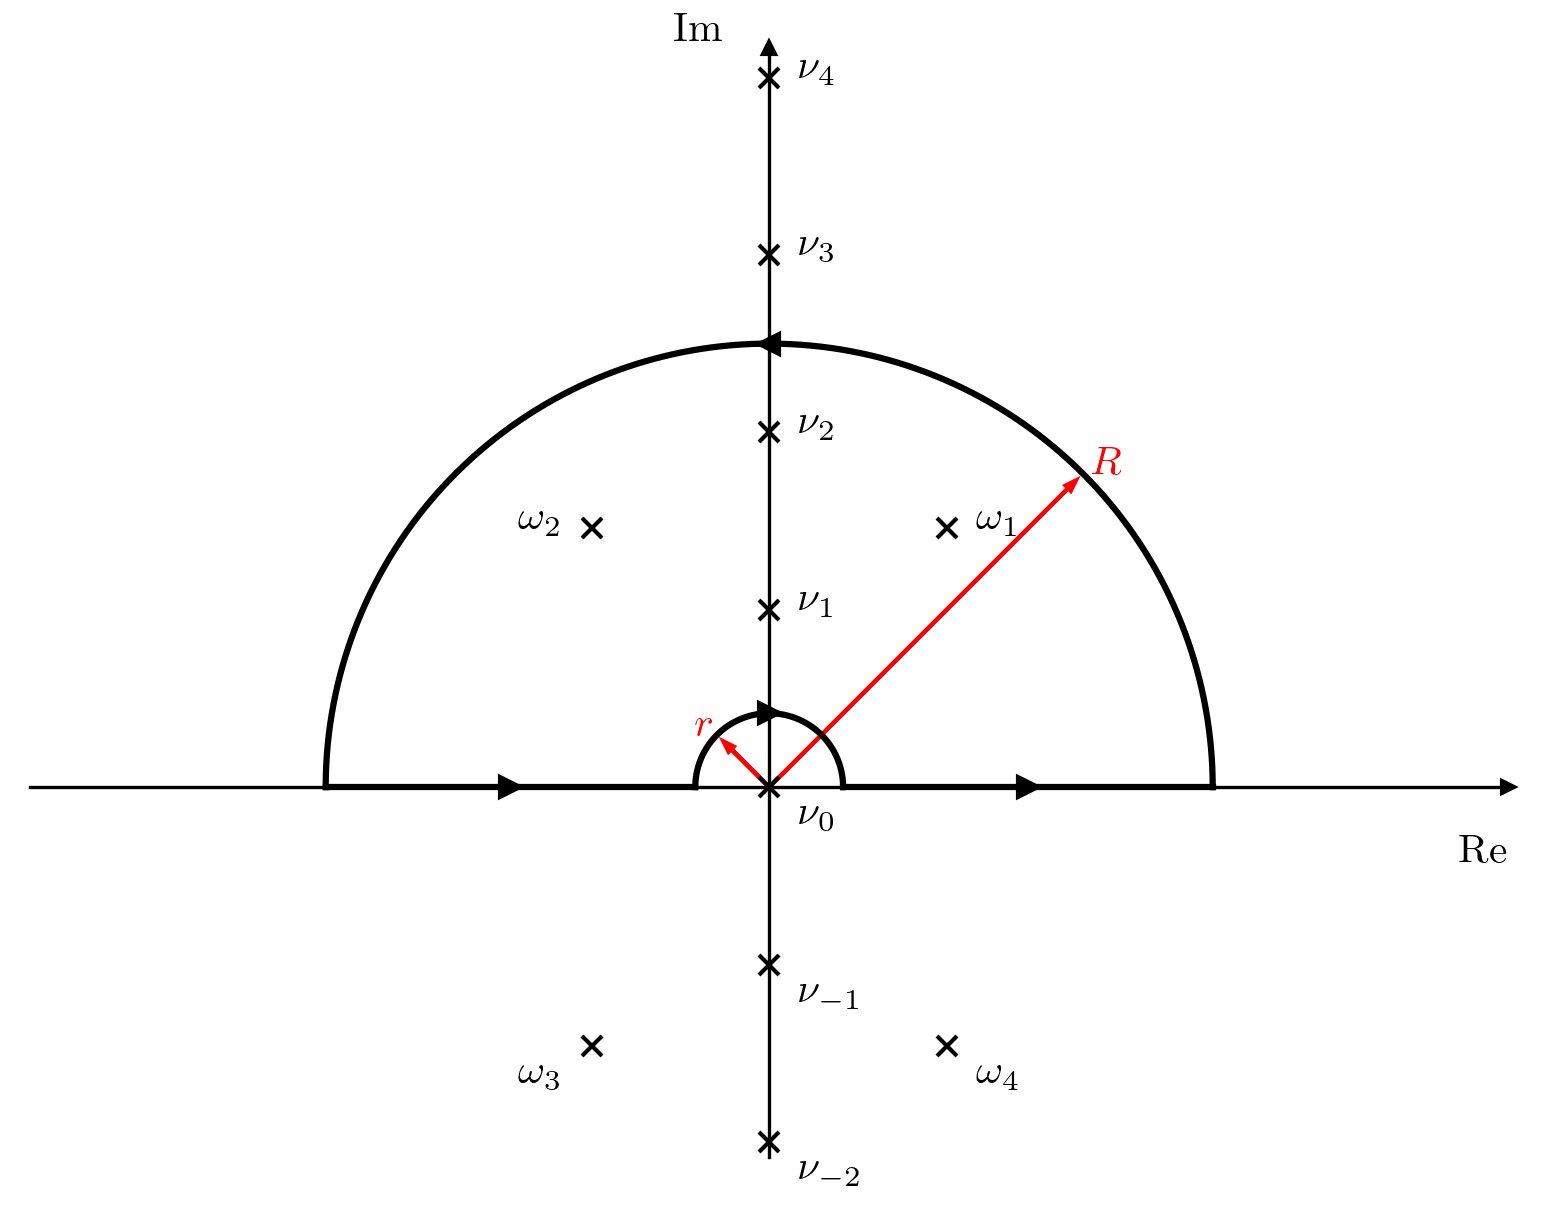
\includegraphics{./images/bath_corr_int_contour.png}

%
\begin{dmath}
    S \left( \tau \right) = 2\pi\alpha \left[ \frac{(\tilde{\Omega}^2+\Gamma^2/4)^2}
    {2\text{i}\tilde{\Omega}\Gamma(\tilde{\Omega}+\text{i}\Gamma/2)(2\tilde{\Omega}+\text{i}\Gamma)}
    \coth\left( \frac{\hbar\beta}{2} \left(\tilde{\Omega}+\text{i}\Gamma/2\right) \right) 
    \left( 1- e^{\text{i}\tilde{\Omega}\tau} e^{-(\Gamma/2) \tau} \right) \\
    + \frac{(\tilde{\Omega}^2+\Gamma^2/4)^2}
    {(-2\text{i}\tilde{\Omega}\Gamma)(-\tilde{\Omega}+\text{i}\Gamma/2)(-2\tilde{\Omega}+\text{i}\Gamma)} 
    \coth\left( \frac{\hbar\beta}{2} \left(-\tilde{\Omega}+\text{i}\Gamma/2\right) \right) 
    \left( 1- e^{-\text{i}\tilde{\Omega}\tau} e^{-(\Gamma/2) \tau} \right) \\
    + \frac{2}{\hbar\beta} \sum_{n=1}^{\infty}\frac{(\tilde{\Omega}^2+\Gamma^2/4)^2}{\text{i}\nu_n
    (\text{i}\nu_n -\tilde{\Omega}-\text{i}\Gamma/2)(\text{i}\nu_n +\tilde{\Omega}-\text{i}\Gamma/2)
    (\text{i}\nu_n +\tilde{\Omega}+\text{i}\Gamma/2)(\text{i}\nu_n -\tilde{\Omega}+\text{i}\Gamma/2)}
    (1-e^{-\nu_n\tau}) \right]
\end{dmath}
%